To gather contextual information about the flagged vulnerable functions, the chosen method was to identify which other functions were their callers and callees. This required generating and analyzing the call graph of the code. A call graph is a representation of a program in the form of a control-flow graph. In this structure:
\begin{itemize}
    \item Each function is depicted as a node.
    \item The relationships between functions, such as function calls, are represented as edges connecting the nodes.
\end{itemize}

This representation reveals how vulnerable functions interact with other parts of the code, facilitating the extraction of contextual information.

For this analysis, the focus was on the PcapPlusPlus project, as it was the only project for which a ground truth vulnerability was detected by a static analysis tool (Infer). To generate the call graph, the \textbf{Static Value-Flow Analysis Framework for Source Code (SVF)}~\cite{svf} was used. SVF is a code analysis tool that enables interprocedural dependence analysis for LLVM-based languages. By providing SVF with a bytecode file generated using the \textbf{LLVM compiler}, the framework produces a .dot file that describes the call graph.

\textbf{LLVM} is an open-source compiler framework widely used for program analysis. It compiles source code into an intermediate representation called LLVM bytecode, which can then be analyzed by tools like SVF. The \texttt{.dot} file generated by SVF serves as a textual representation of the call graph. Figure~\ref{callgraph} illustrates how the \texttt{.dot} formatting translates into a visual representation of a call graph, with nodes representing functions and edges representing calls between them.

\begin{figure}[ht]
    \centering
    \begin{minipage}[t]{0.45\textwidth}
        \vspace{0pt} % Ensure no offset at the start of the minipage
        \begin{lstlisting}
digraph G {
    a [label="Function A"];
    b [label="Function B"];
    c [label="Function C"];
    a -> b;
    a -> c;
}
        \end{lstlisting}
        \vspace{0.5em} % Space between lstlisting and custom caption
        {\footnotesize Call graph in .dot file format.} % Manually add caption text
    \end{minipage}
    \hfill
    \begin{minipage}[t]{0.45\textwidth}
        \vspace{0pt} % Ensure no offset at the start of the minipage
        \centering
        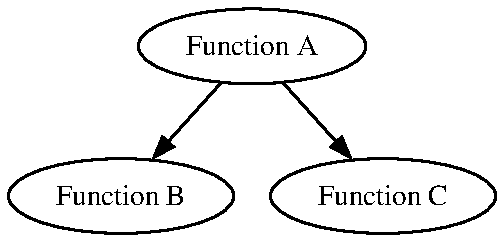
\includegraphics[width=\textwidth]{figures/callgraph.pdf}
        \vspace{0.5em} % Optional space for consistency
        {\footnotesize Graphical representation of the call graph.} % Manually add caption text
    \end{minipage}
    \caption{Comparison of the textual and graphical representation of the call graph.}
    \label{callgraph}
\end{figure}

After generating the call graph, the next step was to filter out the vulnerable functions obtained as described in Subsection~\ref{sec:approach:sub:sast}. This involved:
\begin{enumerate}
    \item Using a Python script to match the function names to the corresponding node labels in the graph. This step was necessary because the nodes in the \texttt{.dot} file are not directly named after the functions, as shown in Figure~\ref{callgraph}.
    \item Performing some manual filtering to address mismatches and inconsistencies in the node labeling.
\end{enumerate}

To navigate the graph and extract callers and callees of the vulnerable functions, the \textbf{pydot} library~\cite{pydot} was used. This Python library efficiently handled the parsing of the \texttt{.dot} file and allowed for the lookup of relevant edges and connected functions, making it easier to analyze the relationships between the nodes.

Once the relevant functions and their contexts were extracted, the results were stored in \texttt{.json} files for further analysis. These files contained details about the vulnerable functions and their relationships with other functions in the graph (e.g., callers and callees). 

After that, the source code for all flagged functions and their related functions were was extracted from the repository and written into separate files, so that it could be sent into the LLM for analysis in the next step.

Despite this focus, only 9 out of the 51 vulnerabilities flagged by Infer in PcapPlusPlus appeared in the call graph generated by SVF, and thus were considered for further analysis. This discrepancy highlights a limitation in the representation or the analysis process, as certain vulnerabilities may correspond to code that was not captured or connected in the generated call graph.
